At some point it was evident, that we spend more and more time on the construction of increasingly complex features. Since this is a machine learning project, we looked for ways to overcome this problem and came up with two possible directions:
\begin{enumerate}
	\item Choosing a different (nonlinear) approximation function, like deep neural networks, decision trees or regression ensembles with gradient boosting.
	\item Finding a way to learn good features (automated feature extraction).
\end{enumerate}
 
We knew from extensive communication with other groups, which opted for option 1, that a change in the approximation function would not be straight-forward. Many more complex function approximators rely on off-policy batch gradient-descent updates and on-policy $n$-step Sarsa and Sarsa($\lambda$) learning algorithms are not applicable at scale. Our initial idea was to implement PCA with training data from the rule based agent, since it is reasonable that the same features resulting in a good performance of the rule based agents might help our agent. A detailed discussion with the group of Fabian Kneissl, revealed that PCA was not applicable here. To explore some new grounds, we read a lot about genetic algorithms for feature selection and extraction with \cite{cha2008}, \cite{nguyen2011} and \cite{li2005} being our primary sources. \\

The key idea, was to rewrite one of our ordinary linear agents, such that its training process depends on a a list of binary expression trees, which each represents a boolean expression. We will call such an agent a \emph{genetic agent}. By default we provide the genetic agent with all of the complex features mentioned above as well as a high number of simple features, e.g. maps representing the agents relative environment up to four tiles in each direction. We will denote this high-dimensional feature vector of a state $s$ by $x(s)$ and call $x(\cdot)$ the \emph{raw features}. All of the boolean expressions represented by the trees, take fixed components of the raw feature vector as input and therefore represent composite features depending on one or multiple raw features. Instead of using all of the raw features for the linear function approximation of the action-value function $q$, the genetic agent now learns with its composite functions. Therefore, the effective number is of features used in the linear regression is no longer the (possibly large) dimension of $x(\cdot)$, but merely the length of the agents list of binary expression trees. \\

\textbf{The problem with simple features.} \\

To give a concrete example, lets assume that the raw feature vector $x(s)$ contains one-hot encoding of the agents surroundings. In a linear model this is only of limited benefit for the agent, since many important situations can not be described well by such a model. If a bomb is one tile above and two tiles to the right from the agent, it is quite possible, that the linear agent will learn to avoid the action \texttt{UP}, since in some situations such a bomb might have killed it. However, in a linear model the agent will shy away from the action \texttt{UP}, even if there is a wall one block above and one block to the right of him, which would block the bomb. If he still chooses the action \texttt{UP}, it is quite possible that the wall to the top right of him adds positive value to the estimation of the \texttt{UP} action. However, this is not desirable if the tile above the agent is blocked. \\

Composite features might fix this problem, by introducing features like \texttt{is tile above free} \texttt{AND} \texttt{(is no bomb in the row above OR will a wall block such a bomb)}, \linebreak where most of the operands are itself composite expressions. Therefore, the aim is to find automatically construct binary expression trees, which represent good features. \pagebreak 

For this complex task, we introduced a genetic algorithm following the following process for feature extraction.

\begin{minipage}{\linewidth}
\begin{center}
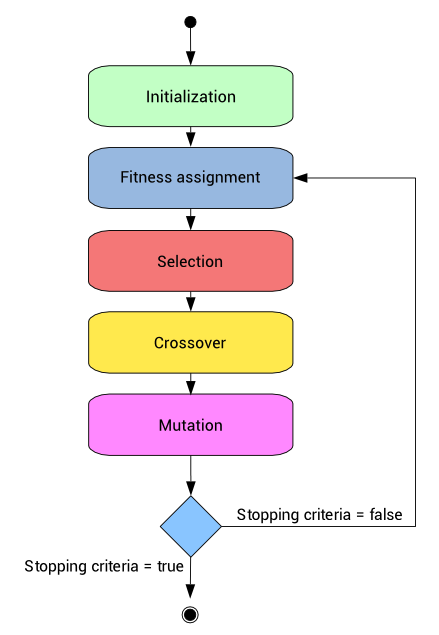
\includegraphics[scale=0.5]{graphics/genetic_algorithm.png}
\captionof{figure}{Modified feature extraction process from \cite{neural_designer}.}
\end{center}
\end{minipage}
\vspace{10pt}

An external script, initializes multiple lists of binary expression trees at random. We will call this set of lists the \emph{population} and one list of binary expression trees an \emph{individual}. Then for each of these individuals the fitness of the associated genetic agent is evaluated by training a linear agent with the corresponding composite features and measuring some kind of performance, e.g. average reward over the last 50 training episodes. After this is done for all the individuals, the best performing agents were selected as \emph{the offspring} and cloned to create a new population. Moreover, on some of the clones mutation and crossover operations were performed. Mutation operations mutate some of the binary trees of an individual at random. Crossover operations take two individuals and exchange whole trees or subtrees. This resulting group of individuals is called the \emph{next generation}. The process is now iterated with the next generation as starting population. Throughout this process, the average performance of the individuals in the population are tracked, which hopefully increases. \\

For the implementation, we used the \texttt{DEAP} \emph{"Distributed evolutionary algorithms in python"} library, which gave us a lot of flexibility and even implemented some standard mutation and crossover operations on binary expressions trees. Using this method, we were able to construct good features in toy examples. One example being the selection of valid game-related features in a raw feature set with many random features (a feature returning 0 or 1 at random). Moreover, the genetic algorithm was able to find solutions to the simple feature problem mentioned above. \\

Unfortunately, there are still multiple flaws with this feature extraction algorithm.
\begin{itemize}
	\item For every new generation, the fitness of each new individual in the population has to be evaluated by training an agent. Since typically many generations are necessary to construct a good features, e.g. a good population, this easily results in long runtimes. 
	\item The genetic algorithm itself introduces a variety of hyperparamters, the primary ones being the population size, the mutation probability, the crossover propbability and the number of generations. Moreover, the concrete choice of mutation and crossover algorithms determines the failure and success of the algorithm. 
\end{itemize}
We tried to use as many heuristics and guidelines mentioned in the sources mentioned above, but in the end the deadline forced us to use our handcrafted features together with a few compound features motivated by the genetic algorithm. Still, the results in toy examples look promising and we are eager to learn more about genetic algorithms for feature extraction in the future. 


